%
% Simple template for generating drafts of papers and articles
%
\documentclass[10pt,]{article}
\usepackage{authblk}
\usepackage{fullpage}
\usepackage{amssymb,amsmath}
\usepackage[utf8x]{inputenc}
\usepackage[T1]{fontenc}
\usepackage{siunitx}
\usepackage[version=3]{mhchem}

\usepackage{natbib}
\bibliographystyle{ametsoc2014}

\usepackage[left]{lineno}
\linenumbers

\usepackage{setspace}
\doublespacing

\usepackage[unicode=true]{hyperref}
\hypersetup{breaklinks=true,
bookmarks=true,
colorlinks=false,
pdfborder={0 0 0}}
\urlstyle{same} % don't use a different (monospace) font for urls

\setcounter{secnumdepth}{5}

\usepackage{graphicx}
\graphicspath{{figures/}}

\makeatletter
\def\ScaleWidthIfNeeded{%
\ifdim\Gin@nat@width>\linewidth
\linewidth
\else
\Gin@nat@width
\fi
}
\def\ScaleHeightIfNeeded{%
\ifdim\Gin@nat@height>0.9\textheight
0.9\textheight
\else
\Gin@nat@width
\fi
}
\makeatother
\setkeys{Gin}{width=\ScaleWidthIfNeeded,height=\ScaleHeightIfNeeded,keepaspectratio}%

% ======================TITLE PAGE=========================

\title{Brain Machine Interface}
\author[1]{Trieu Phat Luu}
\author[1]{Sho Nakagame}
\author[1]{Yongtian He}
\author[1, 2]{Jose L Contreras-Vidal}
\affil[1]{Noninvasive Brain-Machine Interface System Laboratory, Department of Electrical and Computer Engineering, University of Houston, Houston, TX 77004, USA}
\affil[2]{Tecnologico de Monterry, Escuela de Ingenieria y Ciencias, Mexico}

\date{\today}

% ======================CONTENTS===========================

\begin{document}

\maketitle


\newpage
\section*{Abstract}
Write your abstract here.
\newpage

% ======================INTRODUCTION=======================
\section{Introduction}
Paragraph 1. $\theta_{h}$ \textit{BCI-ctrl} $\Delta$ (0.1-3 Hz) $\alpha$/$\mu$ (8-13 Hz)

Paragraph 2.

% ======================METHODS============================
\section{Materials and Methods}
\subsection{Experimental setup and procedure}
Figure \ref{fig:fig_test} shows an example figure.

%==Insert Figure: test.jpg.
\begin{figure}[h]
\noindent
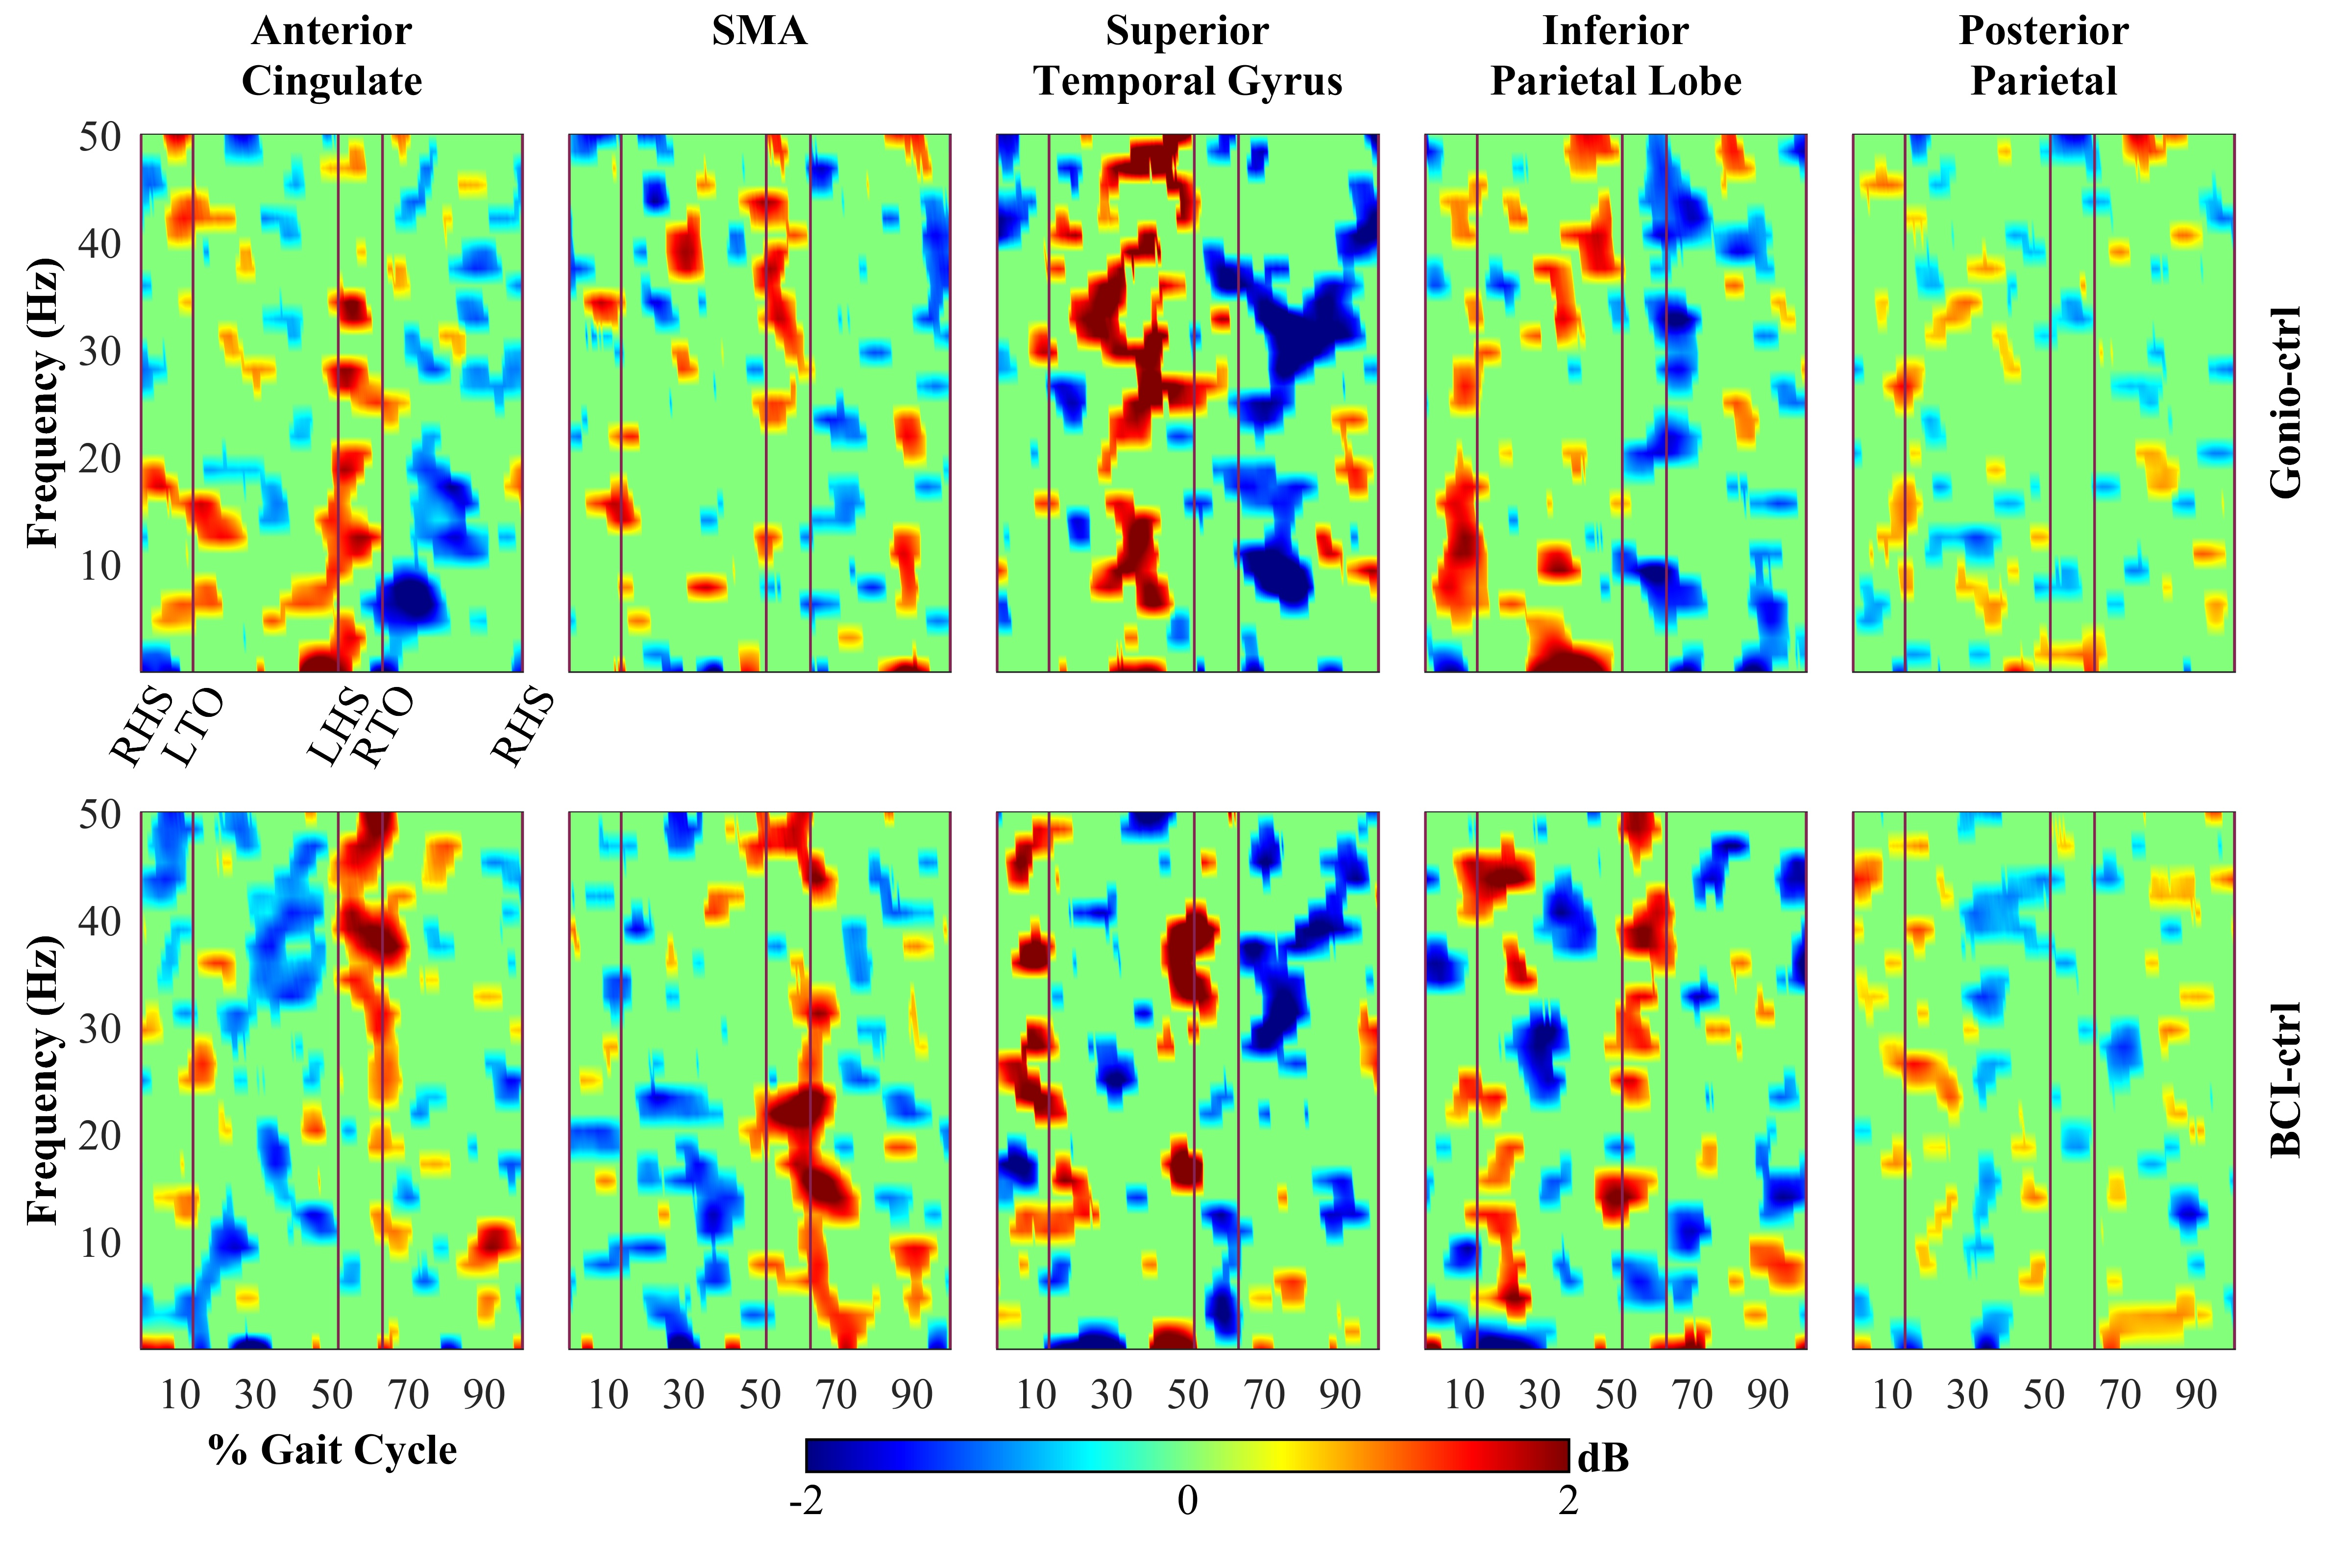
\includegraphics[width=\textwidth]{test.jpg}
\caption{Test figure caption}
\label{fig:fig_test}
\end{figure}
%--

Paragraph 2.

\subsection{Data collection and signal processing for real-time BCI operations}
Paragraph 1.

% ======================RESULTS============================
\section{Results}
\subsection{Result 1}
Paragraph 1.

Paragraph 2.

\subsection{Result 2}
Paragraph 1.
% ======================DISCUSSIONS========================
\section{Discussions}
Paragraph 1.

Paragraph 2.
% ======================REFERENCES=========================
\newpage\clearpage

\renewcommand\refname{References}
\bibliography{xampl.bib}
\newpage

\end{document}

% ======================END================================
